\begin{frame}
   \frametitle{Talk Outline}
   \begin{tikzpicture}[font=\small]
      \tikzset{>=latex} % arrow heads
      \draw[step=1,black!15,very thin,opacity=\gridopacity] (0,0) grid (12,8);

      \node[fill=blue!15,minimum width=11cm] at (6,7.5) {\strut What to Optimize?};

      \node[fill=black!3,minimum width=5cm,minimum height=3cm] (utility) at (3.25,5.6) {};
      \node[anchor=north] at (utility.north) {\strut Maximizing Utility};
      \node at (3.25,5.35) {\includegraphics[width=2.5cm]{build/pvx-utility-anytime}};

      \node[fill=black!3,minimum width=5cm,minimum height=3cm] (family) at (8.75,5.6) {};
      \node[anchor=north] at (family.north) {\strut Utility in C-Space Familes};
      \node at (8.75,5.4) {\includegraphics[width=3.0cm]{build/multiple-sets}};

      \node[fill=blue!15,minimum width=11cm] at (6,3.5) {\strut How to Optimize?};

      \node[fill=black!3,minimum width=5cm,minimum height=3cm] (lazysp) at (3.25,1.6) {};
      \node[anchor=north] at (lazysp.north) {\strut Lazy Pathfinding};
      \node[draw=black!30,fill=white,inner sep=5pt] at (3.25,1.4) {
         \includegraphics[width=3.8cm]{build/lazysp-icon}};

      \node[fill=black!3,minimum width=5cm,minimum height=3cm] (ibid) at (8.75,1.6) {};
      \node[anchor=north] at (ibid.north) {\strut Dynamic Pathfinding};
      \node[draw=black!30,inner sep=0pt] at (8.75,1.4) {
         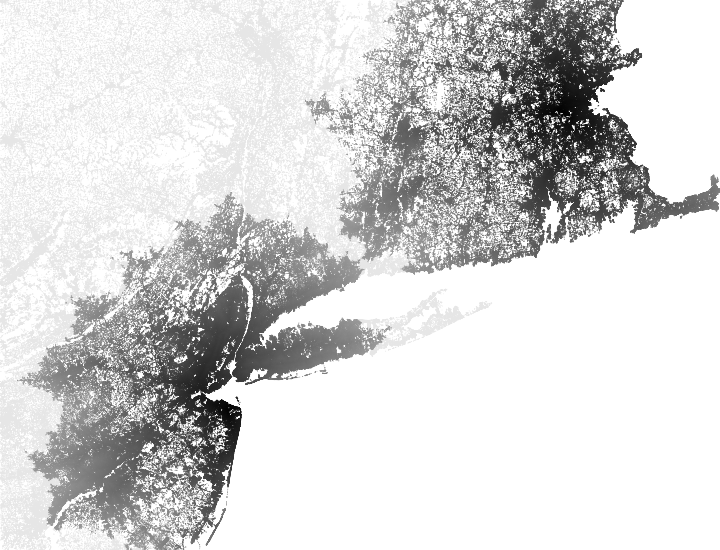
\includegraphics[width=2.9cm]{figs/incbi-road-ne/singleshot/example-bidijkstra.png}};

      \only<2>
      {
         \draw[ultra thick] (utility.north west) rectangle (utility.south east);
      }
      
   \end{tikzpicture}
\end{frame}

%\begin{frame}
%   \frametitle{Maximizing Utility in Motion Planning}
%   \begin{tikzpicture}[font=\small]
%      \tikzset{>=latex} % arrow heads
%
%      \draw[step=1,black!15,very thin,opacity=\gridopacity] (0,0) grid (12,8);
%
%      \node at ( 6,4) {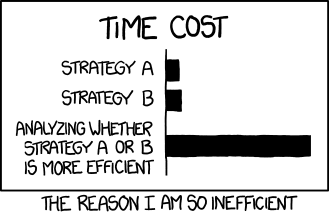
\includegraphics[width=5cm]{figs/xkcd-1445-efficiency.png}};
%      
%   \end{tikzpicture}
%\end{frame}

\begin{frame}
   \frametitle{Maximizing Utility in Motion Planning}
   \begin{tikzpicture}[font=\small]
      \tikzset{>=latex} % arrow heads

      \draw[step=1,black!15,very thin,opacity=\gridopacity] (0,0) grid (12,8);

      \only<1>{\node at (4,5) {\includegraphics{build/pvx-graph-build,drawempty}};}
      \only<2>{\node at (4,5) {\includegraphics{build/pvx-graph-build,drawaxes}};}
      \only<3>{\node at (4,5) {\includegraphics{build/pvx-graph-build,drawa}};}
      \only<4>{\node at (4,5) {\includegraphics{build/pvx-graph-build,drawab}};}
      \only<5>{\node at (4,5) {\includegraphics{build/pvx-graph-build,drawabxstar}};}
      \only<6>{\node at (4,5) {\includegraphics{build/pvx-graph-build,drawabxstarc}};}
      \only<7-8>{\node at (4,5) {\includegraphics{build/pvx-graph-build,drawabxstarcd}};}
      \only<9->{\node at (4,5) {\includegraphics{build/pvx-graph-build,drawabxstarcdutility}};}

      \only<3->{
      \node[fill=blue!5,draw=blue!10,rounded corners,align=center,anchor=north,minimum width=5cm] at (9,6.5) {
         \only<3>{$A_1$: a planner invocation}
         \only<4->{$A_1, A_2$: planner invocations}
         \only<6->{\\ $A_3$: an anytime planner}
         \only<7->{\\ $A_4$: a parameterized planner}};
      }

      \only<2->{
      \node[fill=blue!5,draw=blue!10,rounded corners,align=center] at (4.5,2.0) {
         $p$: planning cost incurred during invocation\\
         $x$: execution cost of resulting solution path};
      }
      \only<8->{
      \node[fill=blue!5,draw=blue!10,rounded corners,align=center] at (4.5,1.0) {
         $U(p,x)$: utility function which scores the invocation};
      }

   \end{tikzpicture}
\end{frame}

\begin{frame}
   \frametitle{Examples of Utility Functions}
   \begin{tikzpicture}[font=\small]
      \tikzset{>=latex} % arrow heads
      \draw[step=1,black!15,very thin,opacity=\gridopacity] (0,0) grid (12,8);

      \only<1->{
      \node at (1.92,6.5) {\includegraphics{build/pvx-sm-firstfeas}};
      \node[anchor=west] at (3.5,6.6) {First Feasible};
      }

      \only<2->{
      \node at (1.82,4.0) {\includegraphics{build/pvx-sm-xbudget}};
      \node[anchor=west] at (3.5,4.1) {Bounded Cost};
      }

      \only<3->{
      \node at (1.92,1.5) {\includegraphics{build/pvx-sm-pbudget}};
      \node[anchor=west] at (3.5,1.6) {Planning Budget};
      }

   \end{tikzpicture}
\end{frame}

\begin{frame}
   \frametitle{General Path Algorithm}
   \begin{tikzpicture}[font=\small]
      \tikzset{>=latex} % arrow heads
      \draw[step=1,black!15,very thin,opacity=\gridopacity] (0,0) grid (12,8);

      \node[fill=blue!5,rounded corners,anchor=north,minimum width=9.5cm,minimum height=3.3cm] (alg) at (6,7.75) {};
      \node[left=0.1cm of alg.north,anchor=north] {\begin{minipage}{9cm}
         \begin{algorithmic}[1]
         \For {iteration $i \in 1, 2, \dots$}
            \State $\bar{p}_i \leftarrow$
               planning cost incurred so far
            \State $\Xi_i \leftarrow$ set of paths to consider at iteration $i$
            \State $\grave{p}_i : \Xi_i \rightarrow \mathbb{R}^+$
               \Comment additional planning cost estimator
            \State $\hat{x}_i : \Xi_i \rightarrow \mathbb{R}^+$
               \Comment execution cost estimator
            \State $\xi_i = \argmax_{\xi \in \Xi_i}
               U\!\left( \; \bar{p}_i \! + \! \grave{p}_i(\xi), \; \hat{x}_i(\xi) \; \right)$
               \label{line:outline-argmax}
            \State \Return $\xi_i$
               if $\xi_i$ fully evaluated, i.e. $\grave{p}(\xi) = 0$
            \State evaluate $\xi_i$
               \Comment incurs requisite planning cost
         \EndFor
         \end{algorithmic}
      \end{minipage}};

      \only<1>{\node at (6.0,2.0) {\includegraphics{build/p-estimates}};}
      \only<2>{
      \node at (3.0,2.0) {\includegraphics{build/pvx-rrt}};
      \node at (9.0,2.0) {\includegraphics{build/rrt}};
      }

   \end{tikzpicture}
\end{frame}

\begin{frame}
   \frametitle{Maximizing Utility on Roadmaps}
   \begin{tikzpicture}[font=\small]
      \draw[step=1,black!15,very thin,opacity=\gridopacity] (0,0) grid (12,8);

      %\node[fill=blue!15,minimum width=11cm] at (6,7.5) {\strut How to Optimize?};
      %\node[fill=blue!15,minimum width=11cm] at (6,6.75) {\strut What to Optimize?};

      \node[fill=blue!5,rounded corners,anchor=north,minimum width=9.5cm,minimum height=3.3cm] (alg) at (6,7.75) {};
      \only<2->{
         \node[fill=blue!20,below=0.83cm of alg.north,minimum width=9.5cm,minimum height=0.4cm] {};
      }
      \node[left=0.1cm of alg.north,anchor=north] {\begin{minipage}{9cm}
         \begin{algorithmic}[1]
         \For {iteration $i \in 1, 2, \dots$}
            \State $\bar{p}_i \leftarrow$
               planning cost incurred so far
            \State $\Xi_i \leftarrow$ set of paths to consider at iteration $i$
            \State $\grave{p}_i : \Xi_i \rightarrow \mathbb{R}^+$
               \Comment additional planning cost estimator
            \State $\hat{x}_i : \Xi_i \rightarrow \mathbb{R}^+$
               \Comment execution cost estimator
            \State $\xi_i = \argmax_{\xi \in \Xi_i}
               U\!\left( \; \bar{p}_i \! + \! \grave{p}_i(\xi), \; \hat{x}_i(\xi) \; \right)$
               \label{line:outline-argmax}
            \State \Return $\xi_i$
               if $\xi_i$ fully evaluated, i.e. $\grave{p}(\xi) = 0$
            \State evaluate $\xi_i$
               \Comment incurs requisite planning cost
         \EndFor
         \end{algorithmic}
      \end{minipage}};

      \only<3->{
         \fill[white,path fading=fade down] (1,6.5) rectangle (11,6.0);
         \fill[white] (1,6.0) rectangle (11,4);

         \node at (2.25,3.25) {\includegraphics[width=3.0cm]{build/roadmap-stack-onramps}};

         \node[anchor=north,fill=black!3,rounded corners] at (8,5.5) {\begin{minipage}{7cm}
            \raggedright
         
            Focus: Roadmap methods

            \medskip
            Advantages:
            \begin{itemize}
            \item Well-studied asymptotic completeness\\
               and optimality properties
            \item Easy to progressively densify
            \item Common structure across queries\\
               (can load roadmaps from disk)
            \end{itemize}
         \end{minipage}};
      }
      
   \end{tikzpicture}
\end{frame}

\begin{frame}
   \frametitle{Maximizing Linear Utilities over Additive Estimators}
   \begin{tikzpicture}[font=\small]
      \draw[step=1,black!15,very thin,opacity=\gridopacity] (0,0) grid (12,8);
      \tikzset{>=latex} % arrow heads

      %\node[fill=blue!15,minimum width=11cm] at (6,7.5) {\strut How to Optimize?};
      %\node[fill=blue!15,minimum width=11cm] at (6,6.75) {\strut What to Optimize?};

      \node[fill=blue!5,rounded corners,anchor=north,minimum width=9.5cm,minimum height=3.3cm] (alg) at (6,7.75) {};
      \only<2->{
         \node[fill=blue!20,below=1.99cm of alg.north,minimum width=9.5cm,minimum height=0.43cm] {};
      }
      \node[left=0.1cm of alg.north,anchor=north] {\begin{minipage}{9cm}
         \begin{algorithmic}[1]
         \For {iteration $i \in 1, 2, \dots$}
            \State $\bar{p}_i \leftarrow$
               planning cost incurred so far
            \State $\Xi_i \leftarrow$ set of paths to consider at iteration $i$
            \State $\grave{p}_i : \Xi_i \rightarrow \mathbb{R}^+$
               \Comment additional planning cost estimator
            \State $\hat{x}_i : \Xi_i \rightarrow \mathbb{R}^+$
               \Comment execution cost estimator
            \State $\xi_i = \argmax_{\xi \in \Xi_i}
               U\!\left( \; \bar{p}_i \! + \! \grave{p}_i(\xi), \; \hat{x}_i(\xi) \; \right)$
               \label{line:outline-argmax}
            \State \Return $\xi_i$
               if $\xi_i$ fully evaluated, i.e. $\grave{p}(\xi) = 0$
            \State evaluate $\xi_i$
               \Comment incurs requisite planning cost
         \EndFor
         \end{algorithmic}
      \end{minipage}};

      \only<3->{
         \node[fill=black!3,rounded corners] at (3.0,3.0) {\begin{minipage}{4.9cm}
            We consider \emph{linear utility functions}:
            \vspace{-0.2cm}
            \[
               -U(p,x) = \lambda_U \, p + (1 - \lambda_U) \, x
            \]
         \end{minipage}};
      }
      \only<5->{
         \node[fill=black!3,rounded corners] at (8.7,3.0) {\begin{minipage}{5.6cm}
            We consider \emph{additive estimators}:
            \vspace{-0.2cm}
            \[
               \xi: \mbox{path on a roadmap graph } G
            \]
            \vspace{-0.5cm}
            \[
               \grave{p}_i(\xi) = \sum_{e \in \xi} \grave{p}_i(e)
               \;\;\mbox{and}\;\;
               \hat{x}_i(\xi) = \sum_{e \in \xi} \hat{x}_i(e)
            \]
         \end{minipage}};
      }

      \only<4>{
         %\node at (9.06,2.25) {\includegraphics[width=3.75cm]{build/pvx-linear-discounting}};
         \node at (8.5,2.25) {\includegraphics[width=3.75cm]{build/pvx-linear-discounting}};
      }

      \only<6->{
         \draw[->,very thick] (5.65,1.9) -- (5.65,1.4);
      
         \node[fill=black!3,rounded corners] at (5.8,0.8) {\begin{minipage}{5cm}
            Shortest path problem with:
            \vspace{-0.2cm}
            \[
               w_i(e) = \lambda_U \, \grave{p}_i(e) + (1 - \lambda_U) \, \hat{x}_i(e)
            \]
         \end{minipage}};
      }
      
   \end{tikzpicture}
\end{frame}

% all this data cumulative over the multistep-prescribed problem

\pgfplotstableread{
lambda searchmean evalmean
lam00 0.13717146918 1.566855428440001
lam20 0.13591121493999997 1.5040972085999997
lam50 0.12633906594 1.3774433666
lam80 0.11458146473999997 1.2423356615
lam99 0.10054155609999996 0.9362152972200001
}{\datasvetimeherbbinnom}

\pgfplotstableread{
lambda searchmean evalmean
lam00 0.9183584741400002 4.73433351068
lam20 0.8734410922000001 4.4884742077799995
lam50 0.82153580024 4.091855509880002
lam80 0.75752757384 3.39455290978
lam99 0.7430251334600001 3.0377397256199994
}{\datasvetimeworkcell}

\begin{frame}
   \frametitle{Search vs. Evaluation Planning Time Comparison}
   \begin{tikzpicture}[font=\small]
      \draw[step=1,black!15,very thin,opacity=\gridopacity] (0,0) grid (12,8);
      \tikzset{>=latex} % arrow heads

      \node at (8.2,7.5) {
         \protect\tikz{\protect\node[fill=red!20,draw=black]{};}\;graph search vs.
         \protect\tikz{\protect\node[fill=blue!20,draw=black]{};}\;edge evaluation
      };

      \node at ( 2.5,5.7) {
         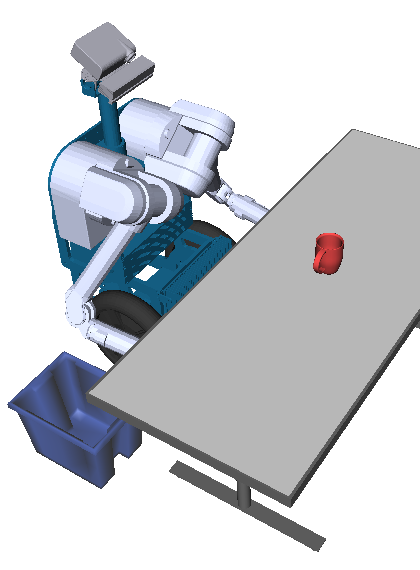
\includegraphics[width=1.7cm]{figs/herbbin/step0cropped.png}
         \;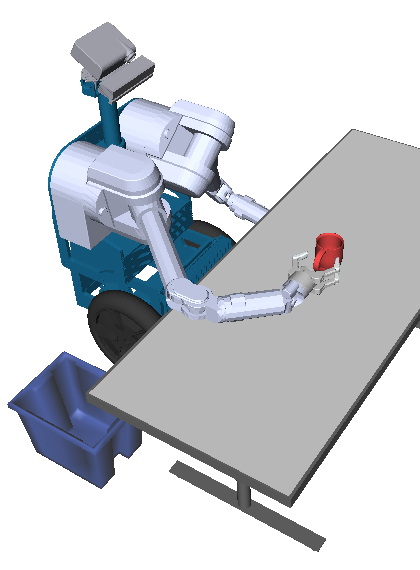
\includegraphics[width=1.7cm]{figs/herbbin/step01cropped.png}};

      \begin{scope}[shift={(5.5,5.0)}]
      \begin{axis}[
         width=7.0cm,
         height=3.2cm,
         xbar stacked,
         bar width=7,
         %xmin=0,xmax=10,
         xmin=0,
         %xtick pos=bottom,
         %symbolic y coords={E, F, R, A, B, W, P},
         %yticklabels from table={\datasvetimeherbbinnom}{lambda},
         yticklabels={$0.00$,,,,$0.99$},
         ylabel={$\lambda$},
         ytick=data,
         %ytick pos=left,
         xmajorgrids,
         xmajorticks=true,
         %ticklabel style={font=\footnotesize},
         enlarge y limits={abs=0.2cm},
         ylabel near ticks,
         ylabel shift=-0.5cm,
         ylabel style={rotate=-90},
         xlabel={Average S/E Planning Time (s)},
         xlabel near ticks,
         ] 
      %\node[circle,fill=white,inner sep=1pt,text=black!40] at (axis cs:40,-5.6) {\scriptsize 40};
      %\node[circle,fill=white,inner sep=1pt,text=black!40] at (axis cs:60,-5.6) {\scriptsize 60};
      %\node[circle,fill=white,inner sep=1pt,text=black!40] at (axis cs:80,-5.6) {\scriptsize 80};
      \addplot[color=black,fill=red!20]
         table[y expr=-\coordindex,x=searchmean]
         {\datasvetimeherbbinnom};
      \addplot[color=black,fill=blue!20]
         table[y expr=-\coordindex,x=evalmean]
         {\datasvetimeherbbinnom};
      \end{axis}
      \end{scope}

      \node at ( 2.5,2.2) {
         \includegraphics[width=3.5cm]{videos/workcell-cropped.png}};

      \begin{scope}[shift={(5.5,1.5)}]
      \begin{axis}[
         width=7.0cm,
         height=3.2cm,
         xbar stacked,
         bar width=7,
         %xmin=0,xmax=10,
         xmin=0,
         %xtick pos=bottom,
         %symbolic y coords={E, F, R, A, B, W, P},
         %yticklabels from table={\datasvetimeherbbinnom}{lambda},
         yticklabels={$0.00$,,,,$0.99$},
         ylabel={$\lambda$},
         ytick=data,
         %ytick pos=left,
         xmajorgrids,
         xmajorticks=true,
         %ticklabel style={font=\footnotesize},
         enlarge y limits={abs=0.2cm},
         ylabel near ticks,
         ylabel shift=-0.5cm,
         ylabel style={rotate=-90},
         xlabel={Average S/E Planning Time (s)},
         xlabel near ticks,
         ] 
      %\node[circle,fill=white,inner sep=1pt,text=black!40] at (axis cs:40,-5.6) {\scriptsize 40};
      %\node[circle,fill=white,inner sep=1pt,text=black!40] at (axis cs:60,-5.6) {\scriptsize 60};
      %\node[circle,fill=white,inner sep=1pt,text=black!40] at (axis cs:80,-5.6) {\scriptsize 80};
      \addplot[color=black,fill=red!20]
         table[y expr=-\coordindex,x=searchmean]
         {\datasvetimeworkcell};
      \addplot[color=black,fill=blue!20]
         table[y expr=-\coordindex,x=evalmean]
         {\datasvetimeworkcell};
      \end{axis}
      \end{scope}

   \end{tikzpicture}
\end{frame}
